\subsection{Análisis de límites}
Para analizar de qué tipo de filtro se trata según la transferencia se calculan los límites para H de s tendiendo a 0 y tendiendo a infinito.

\begin{minipage}{\linewidth}
  \centering
  \begin{minipage}{0.45\linewidth}
    $$\lim_{s \rightarrow 0} H(s) = 0$$
  \end{minipage}
  \hspace{0.05\linewidth}
  \begin{minipage}{0.45\linewidth}
    $$\lim_{s \rightarrow \infty} H(s) = 0.8911$$
  \end{minipage}
\end{minipage}
\vskip0.5cm

Por lo que se concluye que se trata de un filtro pasa altos, pues para las frecuencias cercanas a 0 la ganancia tiende a 0, mientras que para frecuencias altas (tendiendo a infinito) la ganancia es distinta de 0. 

\subsection{Análisis de polos y ceros}
La función de transferencia posee un único cero para $s=0$ y este se trata de un cero de orden 4.

Analizando el denominador se obtiene que la función de transferencia tiene los siguientes polos:
$$
p_{1, 2} = -1136.16 \pm 1374.31 j
$$
$$
p_{3, 4} = -133.34 \pm 939.50 j
$$

Dichos valores se visualizarán en el siguiente diagrama de polos y ceros.

\begin{figure}[H]
    \centering
    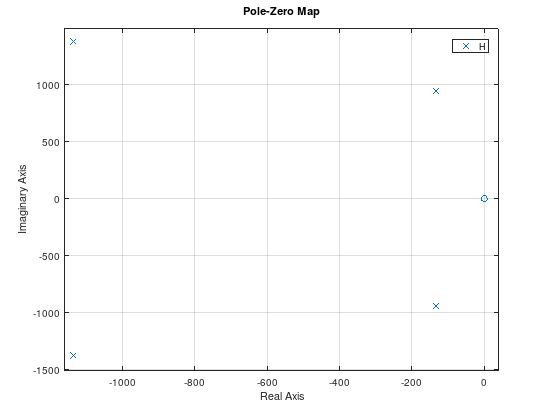
\includegraphics[width=1\textwidth]{resources/pzmap.png}
    \caption{Diagrama de polos y ceros para el circuito}
\end{figure}

Sabiendo esto, podemos descomponer el filtro en dos.

\begin{align*}
    H(s) & = 0.8911 \cdot \frac{s^2}{(s-p_1)\cdot(s-p_2)} \cdot \frac{s^2}{(s-p3)\cdot(s-p4)} \\
         & = \frac{K_1 s^2}{s^2 + 2272.32s+3.17959\cdot10^6} \cdot \frac{K_2 s^2}{s^2+266.68s+900440} \\\\
         & = H_1(s) \cdot H_2(s)
\end{align*}
Con $K_1\cdot K_2 = 0.8911$
\vskip0.5cm
Teniendo en cuenta que los polos denominadores de nuestra transferencia son de la forma  \\$s^2+\frac{\omega_o}{Q}s+\omega_o^2$, se calculará para cada transferencia $H_1$ y $H_2$ cada factor. Siendo entonces:

\begin{itemize}
    \centering
    \item[$H_1$:  ] $\omega_o = 1783.14 $ y $Q = 0.7847$ 
    \item[$H_2$:  ] $\omega_o = 948.91$ y $Q = 3.5583$
\end{itemize}

Ambos valores de Q tienen sentido pues en ambos filtros estamos en presencia de polos complejos conjugados.

\subsection{Análisis de la frecuencia de corte} 
Dado que estamos frente a un filtro pasa altos es oportuno calcular la frecuencia de corte del filtro, es decir la frecuencia $f_o = \frac{\omega_o}{2 \pi}$ tal que la señal se ha atenuado $3dB$, esto es equivalente a que la ganancia máxima se ha reducido en un $29.3\%$. Veamos gráficamente

\begin{figure}[H]
    \centering
    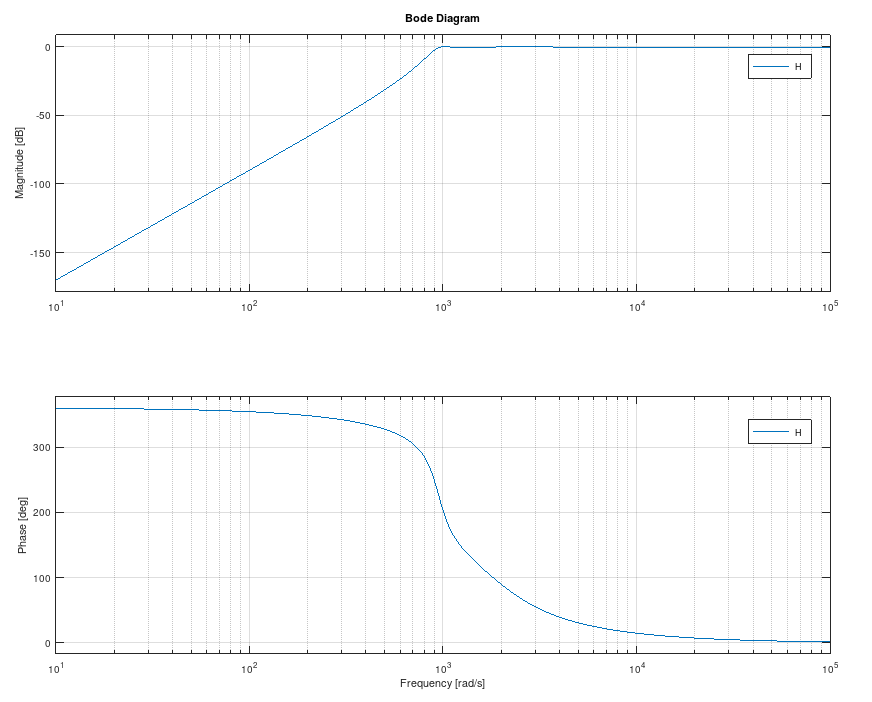
\includegraphics[width=0.8\textwidth]{resources/Bode.png}
    \caption{Diagrama de Bode. En el eje horizontal está la frecuencia angular $\omega$}
\end{figure}

Resolviendo numéricamente (utilizando la biblioteca de sympy en python3) se obtiene el valor para $\omega_o = 895.3 rad/s$, esto se traduce en una frecuencia de corte $f_o = \frac{\omega_o}{2\pi} = 142.4Hz$